\documentclass[11pt]{article}
%\usepackage{fullpage}
\usepackage{epic}
\usepackage{eepic}
\usepackage{paralist}
\usepackage{graphicx}
\usepackage{tikz}
\usepackage{xcolor,colortbl}

\usepackage{fullpage}
\usepackage{amsmath,amsthm,amssymb}
\usepackage{algorithmicx, algorithm}
\usepackage[noend]{algpseudocode}

\newcommand*\Let[2]{\State #1 $\gets$ #2}
\newtheorem{theorem}{Theorem}
\newtheorem{lemma}[theorem]{Lemma}
\newtheorem{proposition}[theorem]{Proposition}
\newtheorem{corollary}[theorem]{Corollary}

\newenvironment{definition}[1][Definition]{\begin{trivlist}
\item[\hskip \labelsep {\bfseries #1}]}{\end{trivlist}}
\newenvironment{example}[1][Example]{\begin{trivlist}
\item[\hskip \labelsep {\bfseries #1}]}{\end{trivlist}}
\newenvironment{remark}[1][Remark]{\begin{trivlist}
\item[\hskip \labelsep {\bfseries #1}]}{\end{trivlist}}


%%%%%%%%%%%%%%%%%%%%%%%%%%%%%%%%%%%%%%%%%%%%%%%%%%%%%%%%%%%%%%%%
% This is FULLPAGE.STY by H.Partl, Version 2 as of 15 Dec 1988.
% Document Style Option to fill the paper just like Plain TeX.

\typeout{Style Option FULLPAGE Version 2 as of 15 Dec 1988}

\topmargin 0pt
\advance \topmargin by -\headheight
\advance \topmargin by -\headsep

\textheight 8.9in

\oddsidemargin 0pt
\evensidemargin \oddsidemargin
\marginparwidth 0.5in

\textwidth 6.5in
%%%%%%%%%%%%%%%%%%%%%%%%%%%%%%%%%%%%%%%%%%%%%%%%%%%%%%%%%%%%%%%%

\pagestyle{empty}
\setlength{\oddsidemargin}{0in}
\setlength{\topmargin}{-0.8in}
\setlength{\textwidth}{6.8in}
\setlength{\textheight}{9.5in}

\setcounter{secnumdepth}{0}

\setlength{\parindent}{0in}
\addtolength{\parskip}{0.2cm}
\setlength{\fboxrule}{.5mm}\setlength{\fboxsep}{1.2mm}
\newlength{\boxlength}\setlength{\boxlength}{\textwidth}
\addtolength{\boxlength}{-4mm}

\newcommand{\algobox}[2]{
  \begin{center}
    \framebox{\parbox{\boxlength}{
        \textbf{Introduction to Algorithms} \hfill \textbf{#1}\\
        \textbf{CS 4820, Spring 2014} \hfill \textbf{#2}}}
  \end{center}}

\newcommand{\algosolutionbox}[2]{
  \begin{center}
    \framebox{\parbox{\boxlength}{
        \textbf{CS 4820, Spring 2014} \hfill \textbf{#1}\\
        #2
      }}
  \end{center}}


\begin{document}


\algosolutionbox{Homework 7, Problem 2}{
  % TODO: fill in your own name, netID, and collaborators
  Name: Piyush Maheshwari\\
  NetID: pm489\\
  Collaborators: None
}

\medskip
\textbf{Hand in your solutions electronically using CMS.
Each solution should be submitted as a separate file.
For multi-part problems, all parts of the solution to that problem should be included in a single file.}

\textbf{Remember that when a problem asks you to design an algorithm, you must also prove the algorithm's correctness and analyze its running time.
The running time must be bounded by a polynomial function of the input size.}

\bigskip

\textit{\textbf{The following problems ask you to design ``self-contained polynomial-time reductions.'' You should interpret that term as follows. If \textsc{a} and \textsc{b} are two decision problems, a self-contained polynomial-time reduction from \textsc{a} to \textsc{b} is a polynomial-time algorithm that takes an instance of \textsc{a} and outputs an instance of \textsc{b}. To show that the reduction is correct, you must prove two things. First, that it transforms \textsc{yes} instances of \textsc{a} to \textsc{yes} instances of \textsc{b}. Second, that it transforms \textsc{no} instances of \textsc{a} to \textsc{no} instances of \textsc{b}.}}

\bigskip

\textbf{(2)}
\emph{(20 points)}
If $G$ is a flow network and $f$ is a flow in $G$,
we say that $f$ \emph{saturates} an edge $e$ if the flow value
on that edge is equal to its capacity, i.e. $f(e) = c_e$.
The \textsc{flow saturation} problem is the following
decision problem: given a flow network $G$ and a positive integer
$k$, determine if there exists a flow $f$ in $G$ such that
$f$ saturates at least $k$ edges of $G$.
This exercise asks you to prove that \textsc{flow saturation} is NP-complete.


\textbf{(a)} \emph{(2 points)}
Show that \textsc{flow saturation} is in NP.


{\bf (b)} { \em (8 points)}
Give a self-contained polynomial-time reduction from \textsc{subset sum} to \textsc{flow saturation}.

{\bf (c)}  {\em (10 points)}
Give a self-contained polynomial-time reduction from \textsc{independent set} to \textsc{flow saturation}.


\subsection{Solution}
\textbf{(a)} A certifier for flow saturation would be the flow $f$ of flow network $G$. If we have the flow, we can check if the flow property is satisfied on every node in $O( V + E)$ time. We can also count the number of edges which are saturated in $O(E)$ time and can verify if atleast k edges have been saturated or not. Hence we can verify the solution in polynomial time in terms of $|V|$ and $|E|$ and hence the Flow Saturation is $NP$.

\textbf{(b)}

Given an instance  of subset sum problem we can construct a flow network $G$ as follows- 

Add a super source $s$ and a super sink $t$. Make nodes $x_1$ to $x_n$ where $n$ is the number of weights in the subset sum problem. Then add two additional nodes $p$ and $q$.

Add edges from $s$ to each $x_i$ of capacity $w_i$. Add edges from all $x_i$'s to $p$ and all $x_i$'s to $q$. Each edge emanating from $x_i$ has weight $w_i$. Then add an edge from $p$ to super sink $t$ with capacity $W$ and add an edge from $q$ to super sink $t$ with capacity INF where INF is any number greater than W.

Also k for this flow network is equal to $2*N + 1$ where n is the number of elements in the subset sum problem.


\begin{center}
\begin{tikzpicture}[scale=0.2]
\tikzstyle{every node}+=[inner sep=0pt]
\draw [black] (11.4,-21) circle (3);
\draw (11.4,-21) node {$s$};
\draw [black] (26.4,-9.5) circle (3);
\draw (26.4,-9.5) node {$x_1$};
\draw [black] (26.4,-17.2) circle (3);
\draw (26.4,-17.2) node {$x_2$};
\draw [black] (26.9,-24.4) circle (3);
\draw (26.9,-24.4) node {$x_3$};
\draw [black] (26.9,-31.9) circle (3);
\draw (26.9,-31.9) node {$x_4$};
\draw [black] (26.4,-38.4) circle (3);
\draw (26.4,-38.4) node {$...$};
\draw [black] (26.4,-46.3) circle (3);
\draw (26.4,-46.3) node {$x_n$};
\draw [black] (53.2,-8.7) circle (3);
\draw (53.2,-8.7) node {$p$};
\draw [black] (55.1,-34.7) circle (3);
\draw (55.1,-34.7) node {$q$};
\draw [black] (71.5,-21.8) circle (3);
\draw (71.5,-21.8) node {$t$};
\draw [black] (13.78,-19.17) -- (24.02,-11.33);
\fill [black] (24.02,-11.33) -- (23.08,-11.42) -- (23.69,-12.21);
\draw (20.5,-15.75) node [below] {$w_1$};
\draw [black] (55.64,-10.45) -- (69.06,-20.05);
\fill [black] (69.06,-20.05) -- (68.7,-19.18) -- (68.12,-19.99);
\draw (60.9,-15.75) node [below] {$W$};
\draw [black] (57.46,-32.85) -- (69.14,-23.65);
\fill [black] (69.14,-23.65) -- (68.2,-23.76) -- (68.82,-24.54);
\draw (65.41,-28.75) node [below] {$INF$};
\draw [black] (29.4,-9.41) -- (50.2,-8.79);
\fill [black] (50.2,-8.79) -- (49.39,-8.31) -- (49.42,-9.31);
\draw (39.77,-8.55) node [above] {$w_1$};
\draw [black] (29.26,-16.29) -- (50.34,-9.61);
\fill [black] (50.34,-9.61) -- (49.43,-9.37) -- (49.73,-10.33);
\draw (41.19,-13.52) node [below] {$w_2$};
\draw [black] (29.48,-22.86) -- (50.62,-10.24);
\fill [black] (50.62,-10.24) -- (49.68,-10.22) -- (50.19,-11.08);
\draw (41.65,-17.05) node [below] {$w_3$};
\draw [black] (29.15,-29.92) -- (50.95,-10.68);
\fill [black] (50.95,-10.68) -- (50.02,-10.84) -- (50.68,-11.59);
\draw (41.66,-20.79) node [below] {$w_4$};
\draw [black] (28.14,-43.86) -- (51.46,-11.14);
\fill [black] (51.46,-11.14) -- (50.59,-11.5) -- (51.4,-12.08);
\draw (40.39,-28.87) node [right] {$w_n$};
\draw [black] (28.96,-18.76) -- (52.54,-33.14);
\fill [black] (52.54,-33.14) -- (52.12,-32.29) -- (51.6,-33.15);
\draw (39.15,-26.45) node [below] {$w_2$};
\draw [black] (29.89,-32.2) -- (52.11,-34.4);
\fill [black] (52.11,-34.4) -- (51.37,-33.83) -- (51.27,-34.82);
\draw (40.7,-33.93) node [below] {$w_4$};
\draw [black] (29.18,-45.18) -- (52.32,-35.82);
\fill [black] (52.32,-35.82) -- (51.39,-35.66) -- (51.76,-36.59);
\draw (42.86,-41.04) node [below] {$w_n$};
\draw [black] (14.33,-21.64) -- (23.97,-23.76);
\fill [black] (23.97,-23.76) -- (23.3,-23.1) -- (23.08,-24.07);
\draw (18.15,-23.33) node [below] {$w_3$};
\draw [black] (13.85,-22.73) -- (24.45,-30.17);
\fill [black] (24.45,-30.17) -- (24.08,-29.31) -- (23.5,-30.12);
\draw (17.55,-26.95) node [below] {$w_4$};
\draw [black] (12.93,-23.58) -- (24.87,-43.72);
\fill [black] (24.87,-43.72) -- (24.89,-42.78) -- (24.03,-43.29);
\draw (18.25,-34.9) node [left] {$w_n$};
\draw [black] (28.65,-11.48) -- (52.85,-32.72);
\fill [black] (52.85,-32.72) -- (52.57,-31.82) -- (51.91,-32.57);
\draw (39.14,-22.59) node [below] {$w_1$};
\draw [black] (29.72,-25.43) -- (52.28,-33.67);
\fill [black] (52.28,-33.67) -- (51.7,-32.93) -- (51.36,-33.87);
\draw (39.52,-30.09) node [below] {$w_3$};
\draw [black] (14.31,-20.26) -- (23.49,-17.94);
\fill [black] (23.49,-17.94) -- (22.59,-17.65) -- (22.84,-18.62);
\draw (20.07,-19.71) node [below] {$w_2$};
\end{tikzpicture}
\end{center}


Now we prove that this is a valid reduction
\begin{proof}
First we prove that a yes instance of this flow network implies a yes instance of the subset sum problem. We have a black box which answers the question - Is there a flow network which saturates atleast k = 2N + 1 edges. Now the only way to saturate 2N+1 edges is to make sure that all edges that go from $x_i$'s to p and q are saturated. This will also ensure that edges from s to $x_i$ are saturated. Also edge $p-t$ would also have been saturated to ensure than 2N+1 saturated edges (since edge $q-t$ can never be saturated since it has a capacity of INF which is greater than $W$).

We can clearly see that if there are any partially saturated edges from $x_i$'s to p or q, then we can never have 2N+1 fully saturated edges. Some of the edges from $x_i$ will go to p and some will go to q. But all of them would be completely saturated in a yes instance. So clearly the subset of edges which go from $x_i$'s to p forms a subset of weights which sum to W due to flow conservation property at p. Hence a yes instance of the flow saturation instance would imply a yes instance of subset sum problem.\\\\
Now we prove that a yes instance of subset sum problem results in an yes instance of the flow saturation problem. If we have a subset of weights that sum to $W$ then we can construct a flow which saturates atleast k  = 2N +1 edges as follows. Let the flow on edges from s to $x_i$'s be $w_i$ which is equal to their capacity. Let the subset of weights which sums to W be $w_a, w_b .. w_k$. Pick the nodes $x_a, x_b .. x_k$ and pass flow equal to their capacity to node $p$. Then pick the remaining $x_i$'s and pass flow equal to their maximum capacity to q. Clearly there are n nodes from $x_i$'s to p and q which are saturated. Also because sum of $w_a, w_b .. w_k$ is equal to W which is the capacity of edge $p-t$, edge $p-t$ is also saturated. This means that we have k = 2N+1 edges which are saturated and the flow saturation problem will output Yes.\\\\
Finally we prove that the reduction takes polynomial time. The flow network $G$ has total of $V = n+4$ nodes and $E = 3N+2$ edges. Constructing this graph would take $O(V + E)$ = $O(N)$ time which is polynomial in N.

Hence the reduction is valid.
\end{proof}
\newpage
\textbf{(c)}
Given an instance  of \textsc{independent set} problem G = (V,E) and k we can construct a flow network $G'$ as follows- 

Add a super source $s$ and a super sink $t$. For each edge $u-v$ in E add a node $g_{uv}$. For each node v in $V$ add a node in $g_v$ in $G'$.\\\\
Add edges from super source $s$ to $g_{uv}$ with capacity 1. From each node $g_{uv}$ add edges to nodes $g_u$ and $g_v$ with capacity 1. From each node $g_u$ add an edge to super sink $t$ with capacity equal to the degree of node $u$ in the original graph $G$.

Let the value $k'$ for flow saturation 2$|E|$ + k where k is the size of independent set in the original problem.

\begin{center}
\begin{tikzpicture}[scale=0.2]
\tikzstyle{every node}+=[inner sep=0pt]
\draw [black] (9.7,-27.8) circle (3);
\draw (9.7,-27.8) node {$s$};
\draw [black] (27,-40.1) circle (3);
\draw (27,-40.1) node {$...$};
\draw [black] (48.4,-14.5) circle (3);
\draw (48.4,-14.5) node {$a$};
\draw [black] (48.3,-26.8) circle (3);
\draw (48.3,-26.8) node {$b$};
\draw [black] (48.2,-37.9) circle (3);
\draw (48.2,-37.9) node {$c$};
\draw [black] (49.2,-49.4) circle (3);
\draw (49.2,-49.4) node {$d$};
\draw [black] (27,-21.8) circle (3);
\draw (27,-21.8) node {$b-c$};
\draw [black] (65.6,-28.3) circle (3);
\draw (65.6,-28.3) node {$t$};
\draw [black] (26.5,-11.1) circle (3);
\draw (26.5,-11.1) node {$a-b$};
\draw [black] (26.4,-31.5) circle (3);
\draw (26.4,-31.5) node {$a-c$};
\draw [black] (26.1,-50.4) circle (3);
\draw (26.1,-50.4) node {$c-d$};
\draw [black] (12.53,-26.82) -- (24.17,-22.78);
\fill [black] (24.17,-22.78) -- (23.25,-22.57) -- (23.57,-23.52);
\draw (19.26,-25.33) node [below] {$1$};
\draw [black] (29.92,-22.49) -- (45.38,-26.11);
\fill [black] (45.38,-26.11) -- (44.71,-25.44) -- (44.49,-26.42);
\draw (36.97,-24.88) node [below] {$1$};
\draw [black] (29.39,-23.61) -- (45.81,-36.09);
\fill [black] (45.81,-36.09) -- (45.48,-35.2) -- (44.87,-36);
\draw (36.6,-30.35) node [below] {$1$};
\draw [black] (50.74,-16.38) -- (63.26,-26.42);
\fill [black] (63.26,-26.42) -- (62.95,-25.53) -- (62.32,-26.31);
\draw (53.89,-21.89) node [below] {$deg(a)$};
\draw [black] (51.29,-27.06) -- (62.61,-28.04);
\fill [black] (62.61,-28.04) -- (61.86,-27.47) -- (61.77,-28.47);
\draw (56.49,-28.28) node [below] {$deg(b)$};
\draw [black] (50.83,-36.45) -- (62.97,-29.75);
\fill [black] (62.97,-29.75) -- (62.03,-29.7) -- (62.51,-30.57);
\draw (59.99,-33.61) node [below] {$deg(c)$};
\draw [black] (51.04,-47.03) -- (63.76,-30.67);
\fill [black] (63.76,-30.67) -- (62.87,-30.99) -- (63.66,-31.61);
\draw (57.97,-40.26) node [right] {$deg(d)$};
\draw [black] (11.83,-25.69) -- (24.37,-13.21);
\fill [black] (24.37,-13.21) -- (23.45,-13.42) -- (24.16,-14.13);
\draw (19.12,-19.93) node [below] {$1$};
\draw [black] (12.63,-28.45) -- (23.47,-30.85);
\fill [black] (23.47,-30.85) -- (22.8,-30.19) -- (22.58,-31.17);
\draw (17.42,-30.23) node [below] {$1$};
\draw [black] (11.46,-30.23) -- (24.34,-47.97);
\fill [black] (24.34,-47.97) -- (24.27,-47.03) -- (23.46,-47.62);
\draw (17.31,-40.48) node [left] {$1$};
\draw [black] (29.46,-11.56) -- (45.44,-14.04);
\fill [black] (45.44,-14.04) -- (44.72,-13.42) -- (44.57,-14.41);
\draw (37.06,-13.39) node [below] {$1$};
\draw [black] (28.93,-12.85) -- (45.87,-25.05);
\fill [black] (45.87,-25.05) -- (45.51,-24.17) -- (44.92,-24.99);
\draw (36.4,-19.45) node [below] {$1$};
\draw [black] (28.77,-29.67) -- (46.03,-16.33);
\fill [black] (46.03,-16.33) -- (45.09,-16.43) -- (45.7,-17.22);
\draw (38.41,-23.5) node [below] {$1$};
\draw [black] (29.28,-32.35) -- (45.32,-37.05);
\fill [black] (45.32,-37.05) -- (44.69,-36.35) -- (44.41,-37.31);
\draw (36.48,-35.25) node [below] {$1$};
\draw [black] (28.71,-48.92) -- (45.59,-39.38);
\fill [black] (45.59,-39.38) -- (44.65,-39.34) -- (45.14,-40.21);
\draw (38.15,-44.65) node [below] {$1$};
\draw [black] (29.1,-50.27) -- (46.2,-49.53);
\fill [black] (46.2,-49.53) -- (45.38,-49.06) -- (45.43,-50.06);
\draw (37.69,-50.44) node [below] {$1$};
\end{tikzpicture}
\end{center}

Now we prove that this is a valid reduction

\begin{proof}

First we show that an yes instance of flow saturation implies a yes instance of independent set problem. We have a black box which gives us an answer to the question - Is there a valid flow which has atleast $k'$ = 2$|E|$ + k saturated edges? 

First notice that from a node $g_{uv}$ we can only have one outgoing edge with a positive flow of one, since we have to maintain flow conservation at each node. This means that the maximum number of nodes that can be saturated from $g_{uv}$'s to $g_u$'s is $|E|$.

The maximum number of nodes that can be saturated from s to $g_{uv}$ is $|E|$. So for the flow to have 2E+k nodes saturated, we must have atleast k edges from nodes $g_u$ to t saturated. This means that for atleast k nodes of type $g_v$ we must have edges equal to deg(v) coming into it. 

Now notice that if a there was an edge $u-v$ in the original graph G and in the flow network we had positive flow from node $g_{uv}$ to node $g_v$, then the edge $g_u$ to t can never saturate since its the sum of incoming edges can never be equal to deg(u) since edge u-v won't contribute to it. This is equivalent to saying that vertex $u$ will not be picked in the independent sum since we have picked vertex v and there is an edge between them. So if we have a yes instance of flow saturation, them we must have atleast k edges  $g_{v}-t$ saturated. Those nodes v's would be part of the independent set simply because no other vertex with which these vertices share an edge can be part of a saturated edge of the form $g_{v}$-t.\\\\
Now we prove that an yes instance of the independent set problem implies an yes instance to the flow saturation problem. If we have an independent set of size k, this simply means that we have a collection of k nodes, none of which share an edge. So if the independent set is $s_1, s_2..., s_k$, we can simply saturate k edges of the form $g_1$-t, $g_2$-t...,$g_k$-t since we can have edges equal to their degree coming into each vertex. Also we can also saturate the edges $g_{uv}$ to vertexes in the independent set. There would be no conflict since no two nodes sharing an edge is part of the independent set. Finally we can saturate all edges of the form s-$g_{uv}$. Hence if we have an independent set of size k, we can have $k'$ = 2$|E|$ + k edges saturated in the flow network and the flow network instance will return Yes.\\\\
Finally we show that the reduction takes polynomial time. The flow network graph that we have build has $|V'| = 2 + |E| + |V|$. It has edges equal to $|E'| = |E| + 2|E| + |V|$. Since this flow network has polynomial number of vertices and edges, it would take polynomial time to build this graph.

Hence the reduction is complete.
\end{proof}

\end{document}
